\documentclass[11pt]{article}
\usepackage[utf8]{inputenc}
\usepackage[T1]{fontenc}
\usepackage{lmodern}
\usepackage[french]{babel}
\usepackage{amsmath, amsthm, epsfig, amsfonts, amssymb, listings, enumerate, color, hyperref, mdframed}
\usepackage{hyperref}

\usepackage{fancyhdr}
\usepackage{lastpage}
\usepackage{float}

\pagestyle{fancy}
\lhead{Programmation en C}
\chead{}
\rhead{EPFL -- Automne 2017}
\headsep = 24pt
\fancyfoot{}
\rfoot{\thepage\ / \pageref{LastPage}}
\renewcommand{\headrule}{\vbox to 0pt{\hbox to \headwidth{\dotfill}\vss}}
\fancyhfoffset[H]{0pt}
\renewcommand{\footrulewidth}{0pt}

\definecolor{dkgreen}{rgb}{0,0.6,0}
\definecolor{gray}{rgb}{0.5,0.5,0.5}
\definecolor{mauve}{rgb}{0.58,0,0.82}

\definecolor{mygray}{rgb}{0.4,0.4,0.4}
\definecolor{mygreen}{rgb}{0,0.8,0.6}
\definecolor{myorange}{rgb}{1.0,0.4,0}
\lstset{frame=tblr,
  language=[ANSI]C,
  aboveskip=3mm,
  belowskip=3mm,
  showstringspaces=false,
  columns=flexible,
  basicstyle={\small\ttfamily},
%  numbers=left,
  numberstyle=\tiny\color{gray},
  keywordstyle=\color{blue},
  commentstyle=\color{dkgreen},
  stringstyle=\color{mauve},
  breaklines=true,
  breakatwhitespace=true
  tabsize=3
}

\textheight 23cm
\textwidth 16.5cm
\voffset -2.5cm
\hoffset -2cm

\parindent 0cm
\parskip.5\baselineskip

\newcommand\tab[1][1cm]{\hspace*{#1}}


\begin{document}

%========================
\begin{center}{\bf Session d'exercices -- Structures et pointeurs}\\
\textbf{\emph{Echantillonage}}
\end{center}

En traitement du signal, on sait qu'un signal échantilloné a une certaine fréquence d'échantillonage peut être parfaitement reconstruit si la fréquence du signal est strictement inférieure à la moitié de la fréquence d'échantillonage. On appelle cette fréquence maximale la fréquence de Nyquist. Dans cet exercice, nous définirons deux structures représentant les caractéristiques d'un signal sinusoïdal simple et d'un échantillonage et utiliserons ensuite ces structures pour vérifier la théorie en échantillonant des signaux de fréquences diverses. A noter que dans cet exercice, un signal complet est défini comme étant une somme de signaux sinusoïdaux.\\
\\
Si la théorie sous-jacente n'est plus très claire pour vous, vous trouverez des informations sur les pages suivantes : 
\begin{enumerate}
%\href{<my_url>}{<description>}

\item  \href{https://fr.wikipedia.org/wiki/Signal\_sinuso\%C3\%AFdal}{Signaux sinusoïdaux}
\item \href{https://fr.wikipedia.org/wiki/\%C3\%89chantillonnage\_(signal)}{Echantillonage}
\item \href{https://fr.wikipedia.org/wiki/Th\%C3\%A9or\%C3\%A8me\_d\%27\%C3\%A9chantillonnage}{Théorème d'échantillonage}
\end{enumerate}

Si la théorie est claire pour vous, vous pouvez passer aux exercices :

\begin{enumerate}

\item \textcolor{mygreen}{[Difficulté: *]} Structures de base\\
Ecrivez les structure \texttt{Sinusoide} et \texttt{Echantillonage}\\
La première doit contenir 3 champs représentant les 3 constantes inhérentes d'un signal sinusoïdal pur : la fréquence, l'amplitude et le déphasage. La seconde doit contenir 2 champs représentant l'instant auquel l'échantillonage commence et sa fréquence.

\vspace{20pt}

\item \textcolor{mygreen}{[Difficulté: **]} Sinusoïde pure\\
Écrivez la fonction
\begin{center} 
\texttt{double sin\_pure(double t, struct Sinusoide s)}, 
\end{center}
qui prend en argument un réel et une structure Sinusoïde et retourne la valeur de la sinusoïde à un instant t. Si l'utilisation des 3 constantes d'une sinusoïde n'est pas claire, se référer aux pages de théorie plus haut.

\vspace{20pt}

\item \textcolor{mygreen}{[Difficulté: **]} Signal\\
Écrivez la fonction
\begin{center} 
\texttt{double signal(double t, int n, struct Sinusoide signal[n])}, 
\end{center}
qui prend en argument un réel et un tableau de sinusoïdes de taille \texttt{n} et retourne l'évaluation du signal au temps \texttt{t}. Il s'agit donc de sommer les évaluations des sinusoïdes à travers le tableau passé en argument en utilisant la fonction précédente.

\vspace{20pt}

\item \textcolor{mygreen}{[Difficulté: **]} Echantillonnage\\
Écrivez la fonction
\begin{center} 
\texttt{void echantillonne(int n, struct Sinusoide s[n],  
				   struct Echantillonage* echant,
                   int nb\_echant, double echantillons[nb\_echant])}, 
\end{center}
Cette fonction prend en argument un Signal, représenté par un tableau de Sinusoïdes, un Echantillonnage et un tableau de réels où seront stockés les échantillons du signal. Pour ceci, il faut donc évaluer le signal \texttt{nb\_echant} fois en partant du temps \texttt{t0} donné par la structure \texttt{echant} et à une fréquence donnée par la même structure. 


\item \textcolor{mygreen}{[Difficulté: *]} Sinus cardinal\\
Écrivez la fonction
\begin{center} 
\texttt{double sinc(double x)}, 
\end{center}
Qui retourne simplement le sinus cardinal $sinc(x)$ d'un réel passé en argument. Pour rappel, $sinc(x) = sin(\pi * x) / \pi*x$ et $sinc(0) = 1$.

\item \textcolor{mygreen}{[Difficulté: **]} Reconstruction du signal\\
Écrivez la fonction
\begin{center} 
\texttt{double reconstruction(double t, struct Echantillonage echant, int nb\_echant, double echantillons[nb\_echant])}, 
\end{center}
Qui, pour un Echantillonage et un tableau d'échantillons (typiquement calculés au préalable par la fonction \texttt{echantillone}), retourne la valeur du signal reconstruit à l'instant t. Ceci est fait n utilisant la formule standard de reconstruction d'un signal, modifiée pour correspondre à cet exercice :\\
\texttt{valeur[i] = echantillons[i] * sinc(echant.fe * (t-echant.t0) - i );}.\\ 
Il s'agit donc de  sommer ces valeurs à travers le tableau d'échantillons passé en argument.

\end{enumerate}

Une fois toutes ces fonctions écrites, il est temps de les tester.

\textcolor{mygreen}{[Difficulté: ***]} Préparation du \texttt{main()}\\
Afin de vérifier et expérimenter avec le théorème d'échantillonnage, vous devez :
\begin{enumerate}

\item Créer un Signal, somme de sinusoïdales, quelconque. Rapelez-vous qu'un tableau de structures peut être initialisé comme :\\
\texttt{
struct Sinusoide s[] =\{\\
    \t\{ 1.0 , 2.0, 0.0 \}, //première sinusoïde pure\\
    \t\{ 0.5 , 4.0, 0.1 \}  //etc.\\
   \};\\}

\item Créer deux Echantillonnages avec le même temps initial et le même nombre d'échantillons mais avec des fréquences différentes. 
L'un devrait avoir une fréquence d'échantillonnage supérieure à 2 fois la fréquence du signal de base et l'autre une fréquence inférieure. Pour rappel, la fréquence d'un signal sinusoïdal est la fréquence la plus élevée parmi les sinusoïdes pures qui sont sommées. 
Dans l'exemple ci-dessus, le fréquence du signal est donc 4.0 et il faudra donc une fréquence d'échantillonnage supérieure à 8.0.

\item Echantilloner le signal de base à l'aide des deux Echantillonnages et de la fonction \texttt{echantillonne}. Cette opération vous donnera deux tableaux d'échantillons qui serviront pour la suite.

\item Reconstruire le signal de base à l'aide des deux Echantillonnages et de la fonction \texttt{reconstruction}. On vous demande ici de simplement évaluer la reconstruction à un temps quelconque.
Rappelez-vous, cette fonction ne fait qu'évaluer le signal reconstruit en un point et ne crée pas de Signal à proprement parler. Pour visualiser le résultat de la reconstruction complète, il faut donc appeler cette fonction à plusieurs instants et comparer le résultat avec le signal original. C'est le sujet de l'exercice suivant. 
\end{enumerate}

\textcolor{mygreen}{[Difficulté: ***]} Visualisation des résultats\\
Maintenant que vos structures ont été initialisées, vous êtes prêts à tester vos fonctions. Ceci se fera en deux phases :
\begin{enumerate}
\item Commencez par "dessiner" les résultats en texte sous forme de colonnes où chaque ligne contient : le temps t, le signal évalué au temps t et les deux reconstructions au même temps t. Pour ce faire, écrivez une boucle \texttt{for} allant de \texttt{t0} à un temps quelconque et avançant par pas de temps (0.1 par exemple).\\
 On s'attend à quelque chose comme :\\
\texttt{
0.000000   0.189358   0.189358   0.189358\\
0.100000   0.755640   0.755640   0.898548\\
0.200000   0.257756   0.257756   0.273642\\
//etc.\\
}
\textit{Note :} On pourrait également afficher une légende en première ligne, 
quelque chose comme\\
 \texttt{t \tab X(t) \tab X\_I(t) \tab X\_II(t)},\\
mais pour la deuxième partie il faut que l'affichage de contienne que des nombres.

\item Vous allez maintenant vraiment dessiner les courbes de ces signaux à l'aide de \texttt{gnuplot} directement depuis le terminal. Ce programme, présent sur la grande majorité des distributions Linux, lit des fichiers contenant des valeurs numériques et trace des courbes basées sur ces valeurs qui doivent être écrites en colonne. Vous comprenez maintenant pourquoi l'affichage se faisait en colonne au point précédent. Cependant, notre programme affiche simplement ces valeurs dans le terminal, pas dans un fichier. Heureusement, il existe une façon très simple de résoudre ce problème. Dans le terminal, déplacez-vous jusqu'au répértoire contenant votre programme et, si celui-ci s'appelle \texttt{echantillonnage} par exemple, tapez simplement \texttt{./echantillonnage > data.txt}. Cette commande éxécute votre programme et \textit{redirige} sa sortie (l'affichage du point précédent) vers le fichier "data.txt". Vérifiez que l'écriture a fonctionné en tapant \texttt{cat data.txt} ce qui devrait afficher la même chose que votre programme.

Ceci fait, il suffit de taper \texttt{gnuplot} dans le terminal et dans gnuplot de taper : \\
\texttt{
\t > set style data line\\
\t > plot "data.txt" u 1:2 t "signal", "data.txt" u 1:3 t "fe 20",\\
"data.txt" u 1:4 t "fe 10"\\
}
Où vous remplacerez "20" et "10" par les fréquences d'échantillonnages que vous aurez utilisé. Avec un affichage sur 100 points, vous devriez obtenir un graphique similaire à celui-ci :
\begin{figure}[H] 
\centering
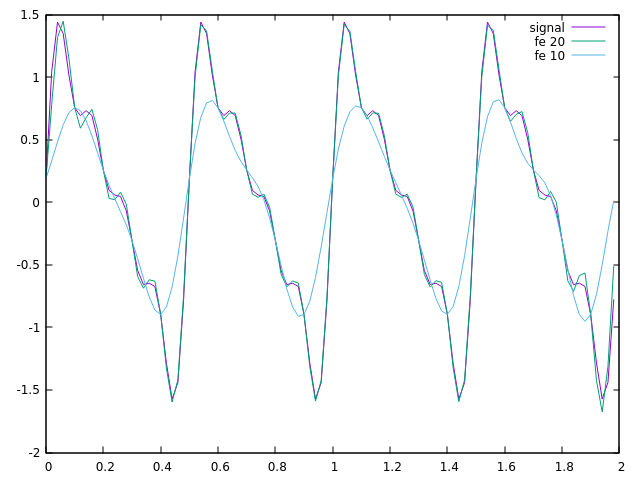
\includegraphics[scale=0.75]{Figures/Result.png}
\end{figure}

Comme vous pouvez le voir, le signal reconstruit à base d'un échantillonage d'une fréquence deux fois supérieure à celle du signal original suit presque parfaitement le signal de base tandis que le second échantillonnage est assez différent. Ceci correspond bien à la théorie et prouve que notre modèle ainsi que notre programme est correct.\\
 \textit{Note :} On remarque que le signal reconstruit ne suit pas exactement la signal de base. Ceci est du au fait que le signal est reconstruit à partir d'une somme finie de sinus cardinaux.

Rapide explication de la commande gnuplot : 
\begin{itemize}
\item Par défaut, gnuplot ne trace que des points. La commande \texttt{set style data line} indique à gnuplot que vous désirez tracer des courbes à la place.
\item \texttt{u 1:2},\texttt{u 1:3} et \texttt{u 1:4} indiquent à gnuplot quelles colonnes utiliser. u 1:3, par exemple indique qu'il faut utiliser la colonne 1 comme abscisse et la colonne 3 comme ordonnée.
\item \texttt{t "signal"}, \texttt{t "fe 10"} et \texttt{t "fe 20"} indiquent simplement la légende à afficher pour chacune des courbes.  
\end{itemize}

Pour plus d'information sur la commande \texttt{plot}, vous pouvez consulter \href{http://www.gnuplot.info/documentation.html}{la documentation officielle} ou taper \texttt{man gnuplot} dans un terminal.

\end{enumerate}



\end{document}